
\chapter{Mineração de Dados} \label{chapter3}

Neste capítulo será apresentada a \textit{mineração de dados} como uma abordagem de apoio para análise de  dados e descoberta de informações. Além do conceito geral, serão apresentados as etapas, técnicas e alguns dos algoritmos utilizados na exploração de dados. A Seção \ref{3title1} apresenta o conceito de mineração de dados e as etapas do processo de extração do conhecimento. A Seção \ref{3title2} apresenta os componentes que constituem um sistema de mineração de dados. A Seção \ref{3title3} apresenta algumas das técnicas de mineração de dados empregadas neste trabalho. A Seção \ref{3title4} lista algumas sugestões de programas \textit{(softwares)} computacionais disponibilizados para análise e mineração de dados, e a Seção \ref{3title5} aborda o \textit{software} Weka, ferramenta utilizada neste trabalho, listando aspectos e recursos disponibilizados pela ferramenta.

\section{Conceitos e Etapas do Processo de Extração do Conhecimento} \label{3title1}

No Capítulo \ref{2title}, foram descritos alguns trabalhos acadêmicos sobre a evasão nos cursos de Computação. Todas as pesquisas consistiram na análise de dados obtidos sobre as Instituições de Ensino, os cursos de graduação e os alunos, de forma a extrair informações que justificassem as taxas elevadas de evasão. No Capítulo \ref{chapter4}, foram apresentados os conceitos de dado, informação e conhecimento, e destacada a importância dos sistemas de gerenciamento de informações para o ambiente organizacional, a fim de facilitar a gestão do conhecimento e potencializar as atividades administrativas através do uso estratégico da informação. 

Com o avanço da tecnologia, várias ferramentas gerenciais foram desenvolvidas para que o processo de análise sobre grandes bases de dados, que podem conter de centenas a milhares de registros, seja realizado de forma automatizada e confiável. A mesma análise, quando realizada de forma manual, torna-se mais susceptível a erros, além de implicar em maiores custos de tempo e recursos, sejam estes humanos ou materiais.
 
Nesse sentido, a mineração de dados \textit{(data mining)} surge como uma metodologia de pesquisa e avaliação, que une conhecimentos e ferramentas da áreas de Computação e Estatística no tratamento de dados e informações e descobertas de padrões de comportamento. Os recursos computacionais disponibilizam algoritmos e \textit{softwares} que buscam otimizar o processo de captura, organização, filtragem, processamento e avaliação dos dados, o que segundo \citet[p. 6]{dantas2014}, \textit{"possibilita a aprendizagem de máquina, elevando a participação dos sistemas computacionais de simples entidades passivas de processamento a entidades com poder de decisão"}. A Estatística, por sua vez, provê subsídios para a interpretação de dados e seus possíveis resultados, tais como análise descritiva, inferência estatística e formas de visualização dos dados.

Na literatura, há várias definições para mineração de dados. \citet[p. 6]{dantas2014} definem como \textit{"o processo de descoberta de vários modelos, resumos e valores derivados de uma determinada coleção de dados".} Já \citet[p. 686]{galvao_marin2009} apresentam a mineração de dados como
\begin{quotation} \textit{"uma das alternativas mais eficazes para extrair conhecimento a partir de grandes volumes de dados, descobrindo relações ocultas, padrões e gerando regras para predizer e correlacionar dados, que podem ajudar as instituições nas tomadas de decisões mais rápidas ou, até mesmo, a atingir um maior grau de confiança".}
\end{quotation}

Embora utilize ferramentas de banco de dados e algoritmos de análise, a mineração de dados, conforme destaca \citet[p. 1-2]{cortes2002}, não é por si só um processo automático, que independe da intervenção humana. Para os autores, a mineração de dados consiste em um
\begin{quotation}
 \textit{"processo altamente cooperativo entre homens e máquinas, que visa a exploração de grandes bancos de dados, com o objetivo de extrair conhecimentos através do reconhecimento de padrões e relacionamento entre variáveis, conhecimentos esses que possam ser obtidos por técnicas comprovadamente confiáveis e validados pela sua expressividade estatística"}. 
\end{quotation}


O apoio ao uso da mineração de dados se estende por diversos motivos, conforme apontados por \citet[\textit{apud} Carvalho (2005)]{amorim2006} e \citet{witten2005}. O crescente volume de dados, a facilidade no armazenamento de dados nos computadores e em rede \textit{(online)}, a necessidade de gerenciamento e padronização dos dados e o atual cenário de competitividade empresarial exigem das organizações um estudo sobre os dados de tal forma que estes possam auxiliar nos processos decisórios, o que pode garantir um maior sucesso ou retorno financeiro para as mesmas. \citet{witten2005} observam que os padrões descobertos pela mineração de dados devem ser significativos, de modo que os resultados possibilitem alguma vantagem ou benefício (geralmente convertidos em benefícios econômicos). 

Para \citet{han_kamber2006}, a análise de informações é uma tarefa que tem ganhado destaque na indústria da informação e na sociedade como um todo, visto que o volume de dados cresce significativamente com o passar dos anos, assim como a necessidade de entendimento sobre os mesmos. A mineração de dados pode ser aplicada a diversos cenários, tais como economia (previsão da variabilidade das taxas de juros), publicidade (pesquisa de opinião, \textit{marketing}, lançamentos de novos produtos), administração (projeções de custos, controle de qualidade), vendas (projeções de vendas, estimativas de lucros), na educação (acompanhamento de resultados de avaliação, projeções de matrículas, estimativas de ingressantes, concluinte e evasão escolar) entre outras. 

Um erro comumente cometido, conforme destacado por \citet{palmeira_santos2014} e também por \citet{cardoso_machado2008}, é a relação de similaridade que se estabelece entre os conceitos de mineração de dados e extração de conhecimento \textit{(KDD - Knowledge-Discovery in Databases)}. A extração de conhecimento consiste na descrição dos processos utilizados para a geração de novos conhecimentos sobre um conjunto de dados, seja para realizar a detecção de novas relações, ou para a descoberta de novos padrões de comportamento ou informações implícitas. \citet[p. 22 \textit{apud} \citet{fayyad1996}]{macedo_matos2010} definem KDD como \textit{"um processo, de várias etapas, não trivial, interativo e iterativo, para identificação de padrões compreensíveis, válidos, novos e potencialmente úteis a partir de grandes conjuntos de dados."} A mineração de dados, por sua vez, é aplicação dos estágios operacionais para estabelecer a descoberta de novos conhecimentos, correspondendo a fase prática do processo.

\citet{fayyad1996} representam o processo operacional de extração de conhecimento (KDD) em cinco estágios, conforme a Figura \ref{fayaad_kdd}, consistindo das seguintes etapas: seleção, pré-processamento, transformação, mineração e interpretação dos dados. 

\begin{figure}[!htb]
\centering
{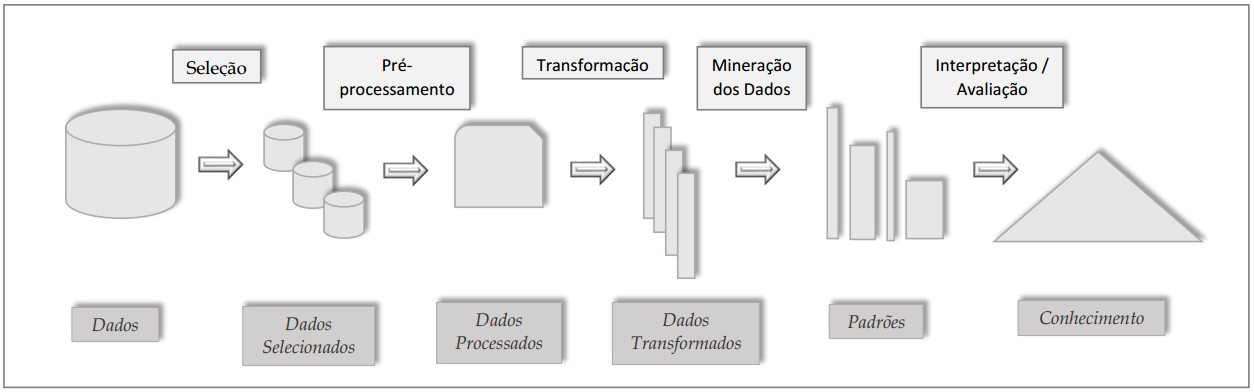
\includegraphics[width=16cm, height=6cm]{images/fases-kdd}}
\caption {Fases do Processo de Extração de Conhecimento (KDD)~\cite{fayyad1996}.}
\label{fayaad_kdd}
\end{figure}

\begin{itemize}
\item \textit{Seleção:} A fase de seleção diz a respeito à análise da disponibilidade e relevância dos dados. É nessa etapa que ocorre a seleção do conjunto ou subconjunto de variáveis ou amostras de dados, onde o processo de descoberta será executado;

\item \textit{Pré-processamento:} A fase de pré-processamento consiste na filtragem e limpeza dos dados. Os processos de filtragem e limpeza visam a remoção de dados inconsistentes, redundantes, valores faltantes ou extremos, que possam interferir nos resultados ou que sejam irrelevantes durante a mineração; 

\item \textit{Transformação:} A fase de transformação consiste na formatação  adequada dos dados, para que os algoritmos possam ser aplicados corretamente. Segundo \citet{han_kamber2006}, a fase de transformação pode envolver as atividades de suavização (remoção de ruídos nos dados),  agregação (sumarização dos dados), generalização (referência por conceitos de fácil entendimento \textit{(alto nível)}), normalização (dimensionamento dos dados em uma faixa de valores) e criação de novos atributos;

\item \textit{Mineração de Dados:} A fase de mineração de dados consiste na exploração e análise dos dados. Nessa fase, são aplicadas as técnicas de mineração de dados, como classificação, sumarização, regressão, clusterização, dentre outras aos atributos, de modo detectar-se padrões de comportamento dos dados e gerar novas descobertas; 

\item \textit{Interpretação e Avaliação:} A fase de interpretação e avaliação, consiste em alcançar propriamente as informações desejadas. Após a finalização da mineração de dados, os resultados obtidos são analisados, sintetizados, avaliados e organizados para apresentação e publicação. 
\end{itemize}

\section{Componentes de um Sistema de Mineração de Dados} \label{3title2}

Segundo \citet{han_kamber2006}, um sistema de mineração de dados é constituído por diversos componentes integrados, conforme a descrição da Figura \ref{componentes}.

\begin{figure}[!htb]
	\centering
	{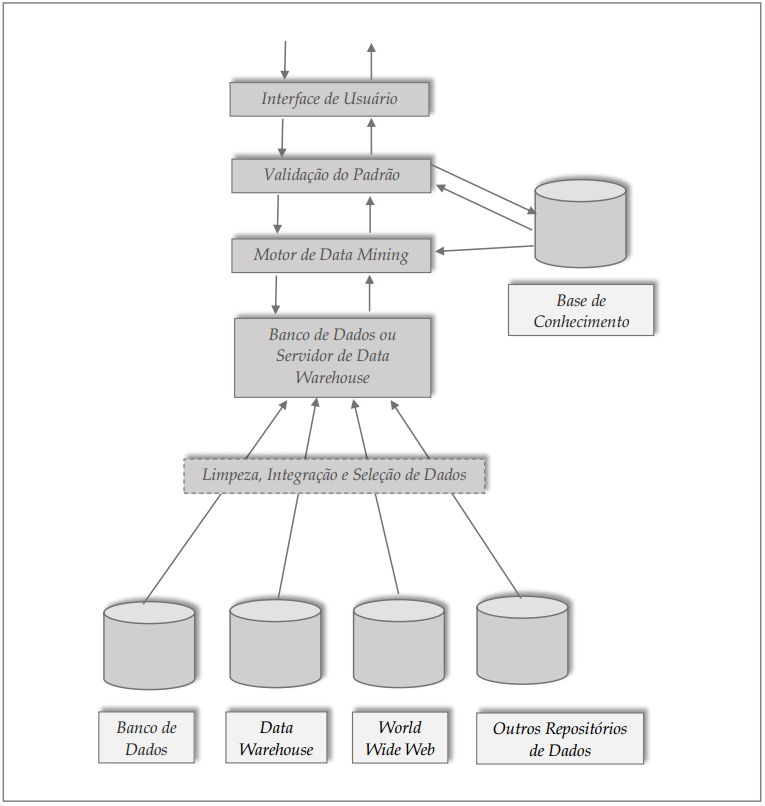
\includegraphics[width=10cm, height=11cm]{images/componentes_mineracao}}
	\caption {Componentes necessários em um sistema de \textit{data mining}~\citep{han_kamber2006}.}
	\label{componentes}
\end{figure}

\begin{itemize}
	\item \textit{Base de aquisição de dados:} podem ser compostos por bancos de dados, \textit{World Wide Web}, repositórios digitais ou \textit{data warehouse};
	
	\item \textit{Servidores de banco de dados ou data warehouse:} tem como função retornar os dados relevantes de acordo com as requisições do usuário;
	
	\item \textit{Base de Conhecimento:} corresponde ao domínio de conhecimento utilizado para orientar a busca dos dados e avaliar os padrões resultantes. Pode fazer uso de hierarquias de conceitos, crenças de usuário, metadados, restrições adicionais ou limites;
	
	\item \textit{Motor de Mineração de Dados:} é essencial na extração de dados. É formado por um conjunto de módulos funcionais que realizam tarefas como caracterização, associação e análise de correlação, classificação, predição, análise de \textit{clusters}, análise de dados ruidosos, entre outras;
	
	\item \textit{Módulo de Avaliação de Padrões:} este componente tem como função empregar medidas e interagir com módulos de mineração de dados com o objetivo encontrar padrões que sejam interessantes (relevantes), sendo possível também utilizar limites para filtrar valores que estejam fora dos padrões. Pode ser integrado ao módulo de mineração de dados, porém deve ser analisado a implementação dos métodos utilizados para mineração de dados;
	
	\item \textit{Interface de Usuário:} este módulo tem por objetivo a comunicação, permitindo a interação entre os usuários e o sistema, dando aos usuários a possibilidade de especificar uma determinada consulta, estabelecer uma tarefa de mineração de dados, inserir informações que aprimorem a pesquisa ou realizar a análise exploratória tomando por base dados intermediários. Entre outras funções, a interface de usuário permite
	a consulta em esquemas de banco de dados, \textit{data warehouse} ou estruturas de dados, avaliar padrões de mineração e visualizar os padrões em formatos diversos.
\end{itemize}

\section{Técnicas de Mineração de Dados} \label{3title3}

Diversas técnicas podem ser empregadas durante o processo de mineração de dados, tais como a classificação, regressão, clusterização, predição, sumarização, detecção de anomalias, dentre outras. Cada técnica fornece uma forma distinta de tratamento e organização dos dados, ficando a critério do avaliador utilizar a(s) que melhor se adequar(em) ao contexto da análise. 

A seguir, serão descritas as técnicas utilizadas na análise de dados neste trabalho, sendo elas a classificação, predição, árvores de decisão, clusterização e detecção de anomalias.

\subsection{Classificação} \label{3subtitle1}

Segundo \citet{han_kamber2006}, classificação é uma forma de análise de dados que extrai modelos que descrevem as classes de dados importantes. \citet{fayyad1996} definem a classificação como a aprendizagem de uma função que mapeia (classifica) um determinado item em uma entre várias classes pré-definidas. \citet[p. 506]{cardoso_machado2008} definem a classificação na mineração de dados como \textit{"o processo de criar modelos (funções) que descrevem e distinguem classes ou conceitos, baseados em dados conhecidos, com o propósito de utilizar esse modelo para predizer a classe de objetos que ainda não foram classificados".}


\citet{han_kamber2006} listam alguns exemplos práticos de classificação na análise de dados. Um agente bancário, durante a realização de um empréstimo, pode utilizar regras de classificação para determinar se um cliente é considerado seguro ou de risco para o banco. O mesmo processo de classificação pode ser utilizado por um gerente de uma loja, para saber o cliente com um determinado perfil pode realizar novas compras; ou por um médico, que pode avaliar dados de determinada doença a fim de prever qual tratamento pode ser mais adequado ou eficaz. 

\citet{han_kamber2006} definem a classificação como um processo de duas etapas. Na primeira fase, um classificador é criado descrevendo o conjunto de dados com classes pré-determinadas, sendo descrito como a \textit{fase de treinamento ou aprendizagem}, onde um algoritmo de classificação cria o classificador analisando ou aprendendo com o conjunto de treinamento. O conjunto de treinamento é uma composição de tuplas geradas pelo banco de dados e seus rótulos de classe associados. Na classificação, uma tupla pode ser constituída por amostras, instâncias, pontos de dados \textit{(data points)} ou objetos de dados. Cada tupla é assumida como pertencente a uma classe pré-definida, sendo determinada pelo atributo do rótulo de classe. Esta etapa também pode ser compreendida como a aprendizagem de um mapeamento ou função pelo classificador (por exemplo, \textit{y = f(t)}, donde \textit{f} pode prever o rótulo de classe \textit{y} de uma determinada tupla \textit{t}).

A segunda etapa consiste na aplicação do classificador sobre o conjunto de dados de teste, composta de tuplas de teste e seus respectivos rótulos de classe. As tuplas de teste são selecionadas aleatoriamente a partir do conjunto de dados geral, e são independentes das tuplas de treinamento, de modo que estas não são usadas na criação do classificador. Nesta etapa, é verificada a precisão (acurácia) do classificador, que é a porcentagem de tuplas do conjunto de testes que foram classificadas corretamente pelo classificador. \citet{han_kamber2006} e  \citet{witten2005} apontam a importância de se mensurar a acurácia do classificador, pois em alguns casos, o classificador pode obter um bom desempenho com dados de treinamento, mas quando aplicado sobre dados de testes, apresentam altas taxas de erro, principalmente quando são analisados dados com algum tipo de ruído (por exemplo, valores desproporcionais ou informados com erro). Caso o classificador apresente resultados considerados satisfatórios, este é considerado apropriado para classificar tuplas de dados cujos rótulos de classes são desconhecidos. 

As duas etapas da classificação são representadas pela Figura \ref{treinamento} (fase de treinamento) e pela Figura \ref{teste} (fase de teste) do classificador sobre as tuplas de dados. 

\begin{figure}[!htb]
	\centering
	{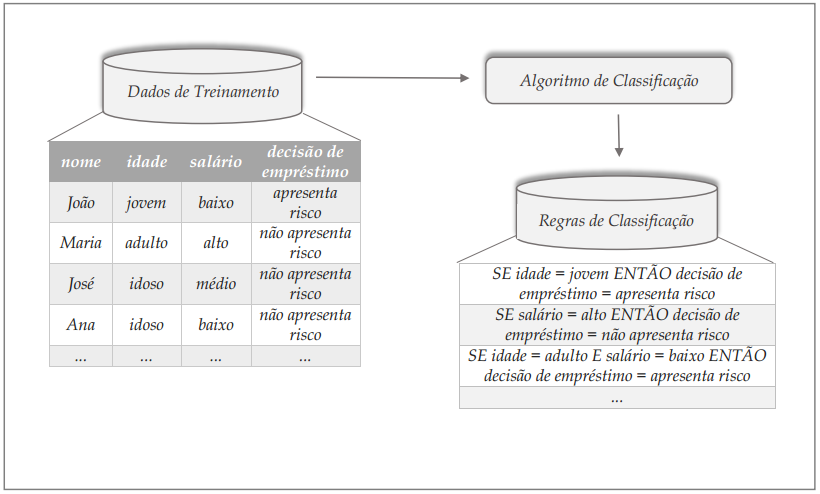
\includegraphics[width=15cm, height=8cm]{images/classificacao1}}
	\caption {Fase de treinamento, onde os dados são analisados por um classificador~\citep{han_kamber2006}.}
	\label{treinamento}
\end{figure}

\begin{figure}[!htb]
	\centering
	{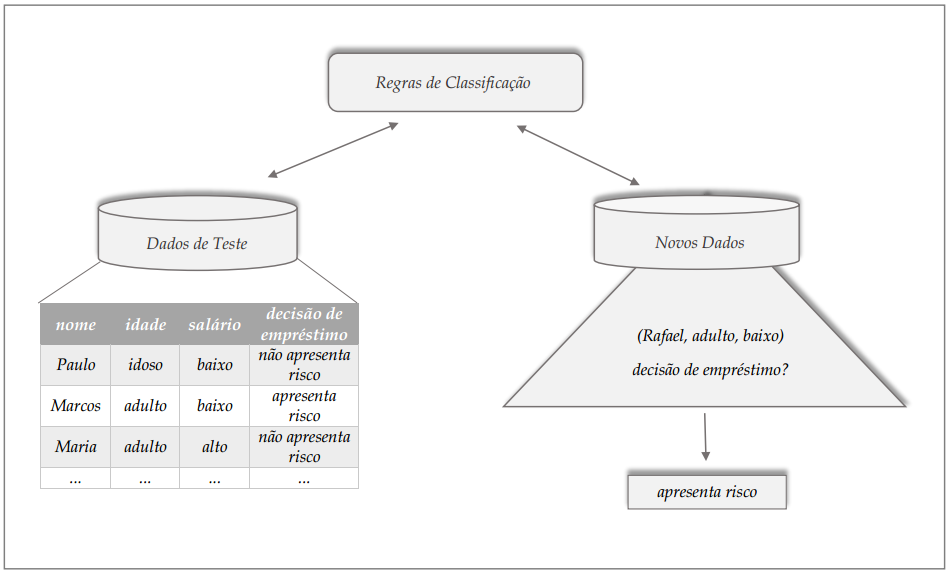
\includegraphics[width=15cm, height=8cm]{images/classificacao2}}
	\caption {Fase de teste, onde os dados de teste são aplicados para estimar a precisão (acurácia) do classificador~\citep{han_kamber2006}.}
	\label{teste}
\end{figure}

\subsubsection{Árvores de Decisão} \label{3subsubtitle3}

Para \citet{coelho_leite}, árvores de decisão são definidas como diagramas elaborados em modo sequencial, baseada em aprendizagem indutiva. \citet{han_kamber2006} definem indução por árvore de decisão como a aprendizagem de árvores de decisão a partir de classes rotuladas nas tuplas de treinamento. A estrutura da árvore de decisão é semelhante a um fluxograma, onde cada nó interno (não-folha) indica um teste de um atributo, cada ramo representa o resultado de um teste e cada nó da folha possui um rótulo de classe. \citet{correa2007} define árvore de decisão como 
\begin{quotation}
	"Uma árvore de decisão é formada por um conjunto de regras de classificação. Cada caminho da raiz até uma folha representa uma destas regras. A árvore de decisão deve ser definida de forma que, para cada observação da base de dados, haja um e apenas um caminho da raiz até a folha." 
\end{quotation}

A Figura \ref{arvore_decisao} apresenta um modelo de árvore de decisão, tomando por base a aprovação do aluno em Computação Básica. Dado que o aluno foi aprovado em Computação Básica, este é classificado como formado. Caso contrário, outras verificações são realizadas na estrutura da árvore, como por exemplo, se o aluno reprovou outras disciplinas. Dada a reprovação do aluno em outras disciplinas,  este é classificado como evadido, e caso contrário, formado.

\begin{figure}[!htb]
	\centering
	{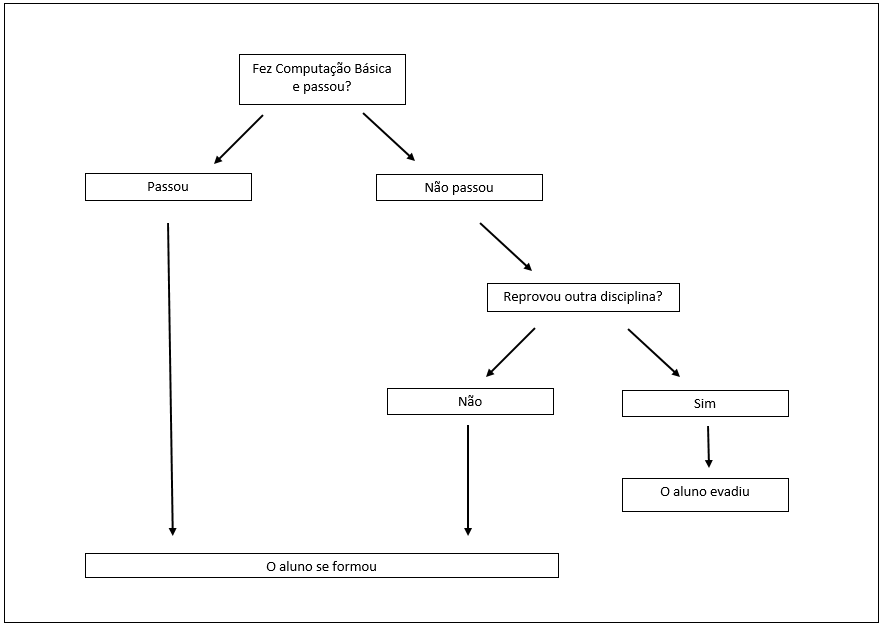
\includegraphics[width=10cm, height=8cm]{images/imagem7}}
	\caption {Exemplo de árvore de decisão.}
	\label{arvore_decisao}
\end{figure}

É importante observar, tomando o exemplo acima, que uma árvore de decisão pode ser usada com dois propósitos: previsão (descobrir se o aluno sairá formado) e descrição (fornecer informações relevantes a respeito da relação entre reprovações na disciplina Computação Básica e o processo de evasão).

Os algoritmos \textit{J48, J48graft} e o \textit{LADTree} são exemplos de algoritmos baseados em árvores de decisão. O algoritmo \textit{J48} gera uma árvore não binária e utiliza uma medida chamada relação de ganho para construir a árvore de decisão, onde o atributo com maior índice de ganho normalizado é tomado como o nó raiz e o conjunto de dados é dividido com base nos valores dos elementos da raiz. O atributo mais relevante é calculado para todos os sub-nós individualmente, e o processo é repetido até que a predição seja concluída. O algoritmo J48 pode lidar com atributos discretos e contínuos, dados de treinamento com valores faltantes e atributos com custos diferentes, além de fornecer uma opção para podar a árvore após sua geração \citep{rajput_arora}. 

O algoritmo \textit{J48graft} é uma versão estendida do J48 que considera a inserção de ramos adicionais para a árvore na fase de pós-processamento. \citet{wisaeng} define a técnica de enxerto como um processo indutivo que adiciona nós inferidos de uma tabela de decisão, com a finalidade de reduzir erros de predição. Ele identifica as regiões no espaço da instância que estão vazias ou contém somente exemplos classificados incorretamente e explora classificações alternativas, considerando diferentes testes que poderiam ter sido selecionados nos nós acima da folha que contém a região em questão \citep{witten2005}. Conforme \citet{rajput_arora}, o propósito é aumentar a probabilidade das instâncias que estão fora do conjunto abrangido pelos dados de treinamento serem classificadas corretamente. Ainda que a árvore torne-se mais complexa, apenas as ramificações (nós) que não introduzam quaisquer erros de classificação em dados já classificados corretamente são considerados.

O algoritmo \textit{LADTree (LAD - Análise Lógica de dados)} é definido por \citet{wisaeng} como um classificador de variável alvo binária, com base na aprendizagem de uma expressão  lógica que pode distinguir amostras positivas e negativas em um conjunto de dados. A construção de um modelo LAD para um conjunto de dados geralmente envolve a geração de amplos padrões estabelecidos e a seleção de um subconjunto que satisfaça a premissa, de modo que cada padrão no modelo satisfaça determinados requisitos em termos de prevalência e homogeneidade. Já \citet{witten2005} descrevem como função do LADTree a construção de multiclasses alternadas de árvores de decisão usando o algoritmo \textit{LogitBoost}.




\subsubsection{Classificação por Regras} \label{3subsubtitle2}

Segundo \citet{han_kamber2006}, a classificação baseada em regras é um modelo representado por um conjunto de regras \textit{'se-então'}, o qual estuda o relacionamento entre itens de dados que ocorrem com frequência, proporcionando a obtenção de associações relevantes em um conjunto de itens aplicados a outros itens e identificando grupos que apresentam uma coocorrência entre si. O condicional \textit{se} de uma regra corresponde ao antecedente da regra ou condição prévia. O condicional \textit{então} corresponde ao resultado da regra. Nas antecedências da regra, a condição pode consistir em um ou mais testes de atributos, e cada regra  pode resultar em uma previsão de classe. A Figura \ref{regras_classificacao} apresenta um exemplo de modelo baseado em regras para classificar um aluno como provável formando em um curso de graduação. A partir dos atributos relacionados à forma de ingresso e idade, foram geradas de regras de classificação para determinar a formatura ou desligamento do aluno.

\begin{figure}[!htb]
	\centering
	{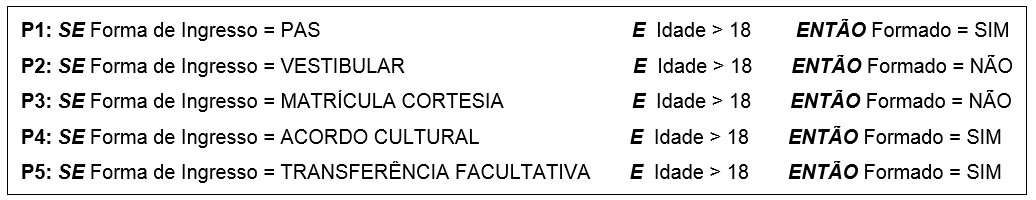
\includegraphics[width=14cm, height=3cm]{images/imagem8}}
	\caption {Exemplo de modelo baseado regras de decisão.}
	\label{regras_classificacao}
\end{figure}

Uma desvantagem apontada por \citet{witten2005} para a geração de regras é o \textit{overfit} (quando o modelo torna-se muito ajustado ao conjunto de dados de treinamento) dos dados de treinamento, não generalizando adequadamente para conjuntos de testes independentes, particularmente em dados ruidosos.  

Os algoritmos \textit{OneR} e \textit{DecisionTable} são exemplos de algoritmos baseados em regras. O algoritmo \textit{OneR}, também conhecido com \textit{1R (uma regra)}, utiliza apenas um dos atributos para realizar a classificação do conjunto de teste. Conforme \citet{zampirolli2014}, o algoritmo consiste, durante a fase de treinamento, em encontrar o atributo que apresente a maior taxa de acerto de classificação das instâncias. Esse algoritmo apresenta um bom desempenho sobre conjunto de dados no qual "um dos atributos é claramente mais importante que o restante, porque seus valores quase sempre darão uma pista de qual deve ser a classificação correta".

O algoritmo \textit{DecisionTable} constrói um classificador com base em tabela de decisão. O algoritmo avalia características de subconjuntos usando pesquisa \textit{best-first} (em tradução livre, primeiro melhor) e pode usar validação cruzada para avaliação. Uma opção utiliza o método \textit{nearest-neighbor} (vizinho mais próximo) para determinar a classe para cada instância que não é abrangida por uma entrada da tabela de decisão, ao invés de utilizar a tabela global, com base no mesmo conjunto de características \citep{witten2005}. 


\subsubsection{Meta-aprendizado} \label{subsubtitle3}

Para \citet[p. 188]{carrier2004}, o  meta-conhecimento consiste em \textit{“qualquer tipo de conhecimento que possa ser extraído da aplicação de um processo de aprendizagem para a resolução de um problema”}. \citet{bezerra2015} definem meta-aprendizado na mineração de dados como uma técnica que visa processar modelos de conhecimento sobre um meta-conhecimento no contexto da mineração de dados. No meta-aprendizado, os algoritmos são ajustados a partir das experiências obtidas de várias aplicações de um algoritmo em fase de treinamento. De acordo com \citet{souza2010}, o meta-aprendizado visa auxiliar a escolha de algoritmos em questões relacionadas a mineração de dados e aprendizagem de máquina, e pode ser utilizado em tarefas de caráter preditivo, tais como classificação. A aplicação do meta-aprendizado em tarefas de classificação é definida como \textit{metaclassificação} \citep{bezerra2015}.

De acordo com \citet{ferrari2014} e \citet{souza2010}, um \textit{meta-exemplo} de treinamento é construído da comparação de um conjunto de algoritmos utilizados em determinado processo de mineração de dados. Cada meta-exemplo é formada por dois conjuntos que armazenam:
\begin{itemize}
	\item (1)- características similares a diferentes instâncias em uma classe (exemplo: número de atributos);
	\item (2)-desempenho dos diferentes algoritmos aplicados ao conjunto de dados.
\end{itemize}

Dado um conjunto de meta-exemplos, um meta-algoritmo é aplicado a fim de verificar as características observadas da mineração e o melhor algoritmo a ser utilizado. O meta-conhecimento obtido sobre os meta-exemplos é utilizado para apontar os algoritmos mais eficientes para situações futuras.

A Figura \ref{meta-classificacao} apresenta o processo simplificado de metaclassificação apresentado por \citet{bezerra2015}. Primeiramente, os classificadores realizam o treinamento no conjunto de dados de treinamento. Em seguida, os classificadores geram predições por meio da análise de um conjunto de teste. A partir do conjunto de teste e das predições geradas, é construído um conjunto de treinamento do meta-nível, e por fim, o metaclassificador gerado é treinado sobre o conjunto de treinamento do meta-nível.

\begin{figure}[!htb]
	\centering
	{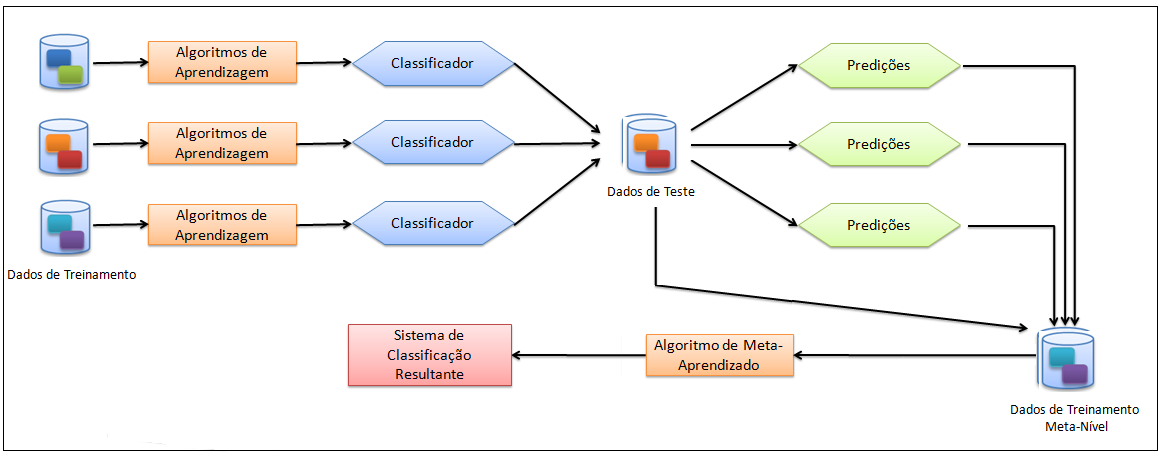
\includegraphics[width=15cm, height=7cm]{images/meta-aprendizado}}
	\caption {Etapas do processo de metaclassificação apresentado por \citet{bezerra2015}.}
	\label{meta-classificacao}
\end{figure}

Os algoritmos \textit{LogitBoost} e \textit{RandomCommittee} são exemplos de algoritmos baseados em meta-aprendizado. O algoritmo \textit{LogitBoost} realiza a regressão logística aditiva. O número apropriado de iterações pode ser determinado por meio de validação cruzada interna \citep{witten2005}. É utilizado para realizar a indução de árvores com modelos de regressão logística linear nas folhas.

O algoritmo \textit{RandomCommittee} constrói um conjunto de classificadores básicos randomicamente e realiza a média de suas previsões. Cada classificador é baseado nos mesmos dados, mas utiliza um número diferente de atributos. Apresenta um bom desempenho desde que a base do classificador seja aleatória, do contrário, todos os classificadores seriam iguais. \citep{witten2005}. 




\subsection{Predição} \label{3subtitle2}

A predição (ou predição numérica) consiste na aplicação de modelos de análise com o objetivo de determinar possíveis valores futuros para um determinado atributo. \citet{han_kamber2006} citam como exemplo um gerente de \textit{marketing} que deseja descobrir quanto um determinado cliente vai gastar durante um processo de venda em uma loja. 

Embora sejam processos similares, vale destacar aqui algumas distinções entre o processo de classificação e predição, conforme apontadas por \citet{han_kamber2006}. Na predição, o classificador consiste em prever valores ordenados, e na classificação rótulos categóricos. A precisão (acurácia), no caso da predição, é estimada calculando o erro com base na diferença entre o valor previsto e o valor efetivo para cada um dos dados do conjunto de teste.

Alguns critérios podem ser levados em consideração para comparar e avaliar os métodos de classificação e predição~\citep{han_kamber2006} a serem utilizados, tais como:
\begin{itemize}
	\item \textit{Acurácia (precisão)}: capacidade de prever corretamente rótulos categóricos ou valores para novos dados;
	
	\item \textit{Velocidade:} referentes aos custos computacionais empregados na geração e utilização de um classificador ou preditor;
	
	\item \textit{Escalabilidade:} capacidade de construir um dado classificador ou preditor de forma eficiente em bases com grandes quantidades de dados;
	
	\item \textit{Robustez:} capacidade de acerto do classificador ou preditor sobre dados com ruídos ou valores faltantes;
	
	\item \textit{Interpretabilidade:} refere-se ao nível de compreensão e entendimento sobre os métodos de classificação e predição. 
\end{itemize}

\subsection{Clusterização} \label{3subtitle4}

Segundo \citet{han_kamber2006}, a clusterização consiste em agrupar um conjunto de objetos, sejam estes físicos ou abstratos, em um grupo de objetos semelhantes. Por sua vez, um \textit{cluster} é definido como um conjunto de objetos de dados que possuem semelhanças entre si e que possuem características distintas em relação a outros conjuntos de objetos, não possuindo classes previamente definidas. A clusterização tem como vantagem a fácil adaptação a mudanças e ajuda a esclarecer características únicas e úteis que possam distinguir diferentes agrupamentos. \citet{han_kamber2006} descrevem que por agrupamento automatizado, é possível identificar regiões densas e esparsas no espaço do objeto, de modo a descobrir padrões globais de distribuição e correlações que sejam interessantes entre os atributos dos dados. A análise de \textit{clusters} pode ser aplicada a vários segmentos, tais como pesquisas de mercado, processamento de imagens e reconhecimento de padrões.

\begin{figure}[!htb]
\centering
{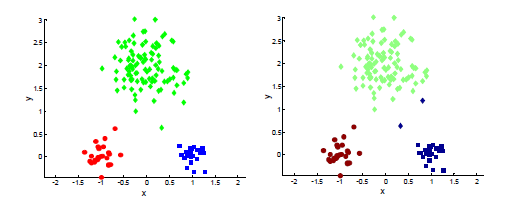
\includegraphics[width=12cm,height=6cm]{images/cluster}}
\caption {Exemplos de agrupamentos de dados \textit{(clusters)}}
\label{cluster}
\end{figure}

Conforme  destacado por \citet{dantas2014}, o processo de clusterização, por vezes, pode ser confundido com o processo de classificação. Na classificação, os objetos são manipulados e distribuídos em classes com características particulares, enquanto que no processo de clusterização os objetos são aglomerados em grupos definidos.

\citet{han_kamber2006} listam alguns requisitos típicos do processo de clusterização em mineração de dados:
\begin{itemize}
\item \textit{Escalabilidade:} muitos algoritmos de clusterização funcionam bem em pequenas bases de dados. No entanto, essas bases também podem conter de centenas a milhares de objetos para análise, o que pode implicar na necessidade de maior desempenho dos algoritmos de análise. Segundo \citet{palmeira_santos2014}, um algoritmo é dito escalável se o tempo de execução do mesmo cresce proporcionalmente ao tamanho do conjunto de dados, considerando os recursos da máquina, como tamanho de memória RAM e processador;

\item \textit{Capacidade de lidar com diferentes tipos de atributos:} os algoritmos devem ser capazes de trabalhar com os mais variados tipos de dados, sejam eles numéricos, nominais, booleanos, dentre outros;

\item \textit{Capacidade de lidar com a alta dimensionalidade dos dados:} um banco de dados pode armazenar registros que contenham várias dimensões ou atributos, o que aumenta o espaço de busca. Dados destas tipologias tornam-se mais difíceis de serem trabalhados, visto que os mesmos podem se encontrar dispersos ou enviesados;

\item \textit{Descobrir \textit{clusters} de forma arbitrária:} muitos algoritmos de agrupamento determinam \textit{clusters} com base em parâmetros de medidas. Baseados nessas medidas, os algoritmos podem reconhecer agrupamentos esféricos com tamanhos e densidades similares. No entanto, um \textit{cluster} pode assumir diferentes formatos, sendo necessário que os algoritmos possam detectar esses agrupamentos de forma arbitrária;

\item \textit{Possuir requisitos mínimos para o domínio de conhecimento para determinar parâmetros de entrada:} os algoritmos geralmente requerem parâmetros de entrada fornecidos pelo usuário para que a análise seja realizada, sendo os resultados  associados aos parâmetros de entrada. Esses parâmetros geralmente são difíceis de serem determinados, principalmente em conjunto de dados que contém objetos de alta dimensão;

\item \textit {Habilidade para lidar com ruídos de dados:} os banco de dados podem fornecer dados com valores extremos, ambíguos ou desconhecidos. Alguns algoritmos, ao trabalhar com estes tipos de dados, tendem a produzir resultados insatisfatórios ou diferentes da realidade;

\item \textit{Possibilitar o agrupamento incremental e insensível à ordem dos registros de entrada:} alguns algoritmos não possibilitam a inserção de novos dados, sendo necessário criar novos agrupamentos. Outros algoritmos são sensíveis à ordem de entrada dos dados, retornando assim agrupamentos diferentes dependendo dos dados de entrada. Daí a importância de algoritmos que sejam incrementais e insensíveis à entrada de novos registros.

\item \textit{Possuir base em restrições de agrupamento:} algumas aplicações trabalhadas no mundo real necessitam de estabelecer restrições sobre os dados, e o principal desafio sobre este aspecto é encontrar agrupamentos de dados que apresentem um bom comportamento sobre as restrições especificadas;

\item \textit{Ser interpretável e utilizável:} os resultados devem ser interpretáveis, compreensíveis e utilizados pelo usuário, onde os agrupamentos estejam relacionados ao contexto das interpretações e aplicações.
\end{itemize}


\subsection{Detecção de Anomalias} \label{3subtitle5}

A detecção de anomalias, também referenciada como detecção de desvios ou análise de \textit{outliers} (valores extremos), visa identificar dados que não se encontram de acordo com os padrões especificados para a mineração, considerados exceções ou ruídos, conforme mostrado na Figura \ref{anomalias}. Estes dados, na maioria das vezes, tendem a impactar de forma negativa os resultados obtidos na mineração de dados.

\begin{figure}[!htb]
\centering
{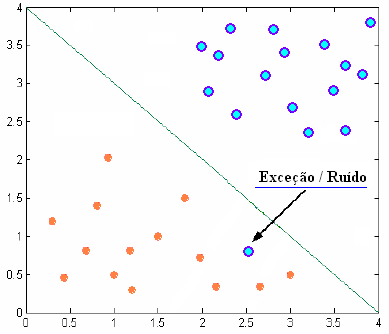
\includegraphics[width=8cm,height=7cm]{images/anomalia}}
\caption {Detecção de anomalia (exceção) no conjunto de dados.}
\label{anomalias}
\end{figure}

A análise e detecção de anomalias permite apresentar novos padrões e alterações de comportamento, tais como atividades suspeitas, potenciais ameaças e possibilidades de fraudes~\citep{witten2005}, contribuindo para o monitoramento e segurança de transações e sistemas. \citet{han_kamber2006} descrevem que no processo de detecção de anomalias, são constituídos modelos de comportamento normal para a rede, que são usados para comparar e identificar novos padrões que se afastam dos perfis pré-definidos. Como vantagem, a detecção de anomalias permite identificar mais claramente ruídos que até então não foram observados, porém apresenta como desvantagem a alta porcentagem de detecção de falsos positivos (por exemplo, uma pessoa saudável é classificada como doente). 

Uma observação importante a ser destacada é que conjunto de regras com muitas especificações também pode induzir o resultado ao erro. Conforme apontado por \citet{miranda2012}, dois aspectos se encaixam nesse cenário: o \textit{overfitting} e o \textit{underfitting}. 

O \textit{overfitting} diz respeito ao alto grau de complexidade dos modelos de regras, apresentando muitos parâmetros relativos ao número de observações. Nestes casos, pode-se ajustar o algoritmo para apresentar um alto grau de precisão para dados conhecidos. Porém, quando aplicados em novos dados, estes tendem a diminuir a precisão dos resultados. \citet{miranda2012} destaca que em situações de \textit{overfitting}, altas taxas de erros são identificadas no retorno dos dados utilizados na base de teste. 

Em contrapartida, o \textit{underfitting} pode ser resultado de um modelo que é demasiadamente simplificado, de tal forma que o algoritmo não consegue se ajustar aos dados. Assim, a probabilidade do algoritmo apresentar altas taxas de erro aumenta, tanto no conjunto de treinamento como no de teste. Ambos os casos devem ser analisados com cautela, pois podem interferir diretamente nos resultados obtidos pelo pesquisador.

\section{\textit{Softwares} para Mineração de Dados} \label{3title4}

No mercado, existem várias ferramentas proprietárias e \textit{open source}\footnote{\textit{Open Source} é o termo utilizado para designar \textit{softwares} de código aberto.}  que auxiliam na mineração de dados, desde a fase de pré-processamento até a visualização dos resultados obtidos. A seguir, serão explanados previamente alguns dos \textit{softwares} abertos que podem ser encontrados e baixados pela Internet \textit{(download)}.

\begin{itemize}

\item \textit{R:} É uma linguagem e ao mesmo tempo um ambiente para a realização de computação que envolvam cálculos estatísticos e gráficos. É semelhante a linguagem S, desenvolvida pela Bell Laboratories (antiga AT \& T, agora Lucent Technologies), embora sejam consideradas diferentes em termos de implementação~\footnote{\url{http://http://www.r-project.org/about.html}}. R fornece uma série de técnicas gráficas e estatísticas (modelos lineares e não-lineares, classificação, clusterização, análise de séries temporais, entre outras) que são altamente extensíveis. Pode ser utilizada e difundida por profissionais de diversas áreas de atuação, tais como economia, medicina e ciência da computação, devido à sua quantidade de materiais bibliográficos disponíveis na Internet. Uma das facilidades oferecidas pelo R é a disponibilização de símbolos e fórmulas matemáticas disponíveis que facilitam na geração e publicação de relatórios. Sua estrutura conta com um conjunto integrado que permite a manipulação e armazenamento de dados, contém operadores para cálculos em tabelas, ferramentas para análise de dados, instalações gráficas que permitem a visualização dos dados em tela ou de forma impressa, além de sua linguagem de programação permitir o uso de condicionais, funções recursivas, estruturas de repetição e manipulação de entrada e saída de dados. É uma ferramenta que está disponível para diferentes plataformas, como Windows, Mac OS e Unix (incluindo o FreeBSD e o Linux).

\item \textit{RapidMiner:} O RapidMiner~\footnote{ \url{https://rapidminer.com/}} é um \textit{software} produzido pela empresa com o mesmo nome, que fornece um conjunto integrado de aplicações que permitem a mineração de dados. É utilizado nos mais diversos contextos, tais como aplicações comerciais, bem como para a investigação, educação, formação, a modelagem e desenvolvimento de aplicativos, e provê suporte para todas as etapas do processo de mineração de dados, incluindo a visualização, otimização e validação dos resultados. Assim como para a mineração de dados, o RapidMiner pode ser aplicado para a aprendizagem de máquina, mineração de textos, análise preditiva e análise de negócios. Este se encontra disponíveis em versões pagas (\textit{Personal Edition} e \textit{Profissional Edition}), e na versão gratuita (\textit{Starter Edition}), que é mais limitada em recursos disponibilizados.

\item \textit{Pentaho:} Pentaho é um \textit{software} desenvolvido em Java, desenvolvido em 2004 pela Pentaho Corporation~\footnote{\url{http://www.pentaho.com/}}. É fortemente utilizado para aplicações que envolvam inteligência empresarial. Sua estrutura é composta por diversos componentes, que permitem realizar a extração, transformação e carregamento dos dados; mineração, análise de \textit{clusters}, processamento de grandes bases de dados; geração de relatórios e metadados.
\end{itemize}

Além das ferramentas listadas acima, outra que é amplamente utilizada no processo de mineração de dados é o \textbf{Weka}, a ser abordada mais detalhadamente na próxima seção, e que será a ferramenta base para o processo de mineração de dados a ser desenvolvido neste trabalho.

\section{\textit{Software} Weka} \label{3title5}

\textit{Weka} é uma abreviação para Waikato Environment for Knowledge Analisys, (em tradução livre, Ambiente Waikato para Análise do Conhecimento), desenvolvido pela Universidade de Waikato, localizada na Nova Zelândia. O \textit{software} é composto por algoritmos de aprendizagem de máquina e uma coleção de recursos que realizam o pré-processamento, regressão, classificação, clusterização, aplicação de regras de visualização dos dados e apresentação de resultados~\citep{weka}. A ferramenta é desenvolvida utilizando a linguagem de programação Java e sua distribuição segue os termos da GNU \textit{(General Public Licence, ou Licença Pública Geral)}. 

O Weka apresenta uma variedade de recursos e ferramentas, como amplo suporte a todas as etapas do processo experimental de mineração de dados, desde a preparação dos dados de entrada, análise estatística de esquemas de aprendizagem até a visualização dos dados e apresentação dos resultados. Possui uma variedade de algoritmos de treinamento e ferramentas de pré-processamento, que são apresentadas em uma interface amigável ao usuário, além de possibilitar a integração direta com bancos de dados, o que permite ao usuário obter os dados direto da base e salvá-los em formato adequado para uso posterior no Weka. Outra vantagem é que a ferramenta é de distribuição livre e multiplataforma, funcionando em diferentes sistemas operacionais, como Windows, Linux e Mac OS. A Figura \ref{weka} apresenta a interface de usuário inicial do Weka.

\begin{figure}[!htb]
	\centering
	{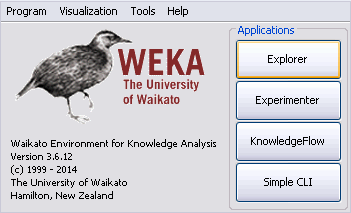
\includegraphics[width=9cm,height=6cm]{images/weka}}
	\caption {Interface inicial do Weka.}
	\label{weka}
\end{figure}


De acordo com \citet{witten2005}, o Weka pode ser trabalhado utilizando as interfaces gráficas \textit{Explorer}, \textit{Experimenter} e \textit{KnowledgeFlow}. 

A interface \textit{Explorer}, mostrada na Figura \ref{modo1}, oferece ao usuário a possibilidade de acesso às opções existentes na barra de menu, assim como possibilita ao usuário carregar os dados a serem utilizados e a verificar os resultados gerados pelos algoritmos de mineração. Porém, uma das desvantagens do modo \textit{Explorer} é que todo o conjunto de dados utilizado é mantido em memória, limitando-se a problemas de pequeno e médio porte.

\begin{figure}[!htb]
	\centering
	{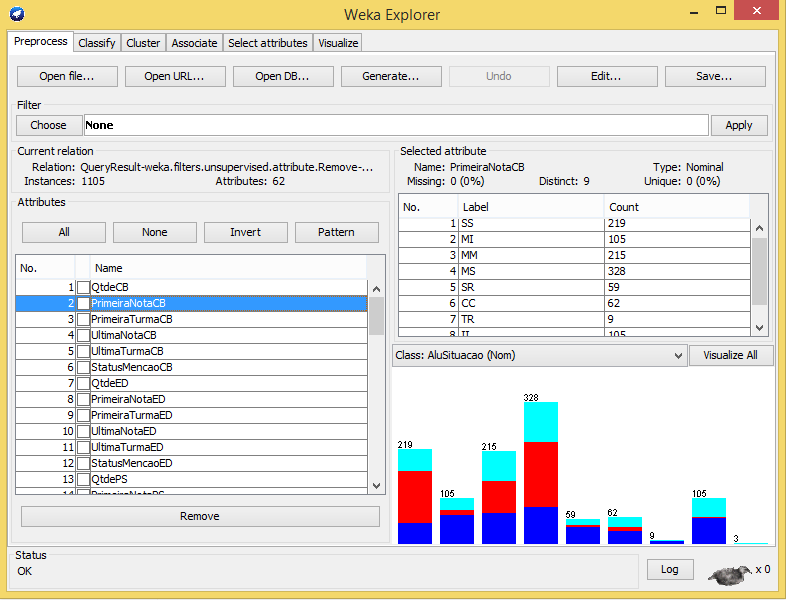
\includegraphics[width=10cm,height=7cm]{images/modo1}}
	\caption {Captura de tela da interface \textit{Explorer} do Weka.}
	\label{modo1}
\end{figure}


A interface \textit{KnowledgeFlow}, mostrada na Figura \ref{modo2}, permite a criação de configurações para o processamento de fluxo de dados. Pela interface gráfica do \textit{KnowledgeFlow}, é possível arrastar caixas que representam os algoritmos de aprendizagem e fontes de dados ao redor da tela, e juntá-los na configuração desejada. Também permite especificar um fluxo de dados por componentes conectados que representam  as fontes de dados, ferramentas de pré-processamento, algoritmos de mineração, métodos de avaliação e módulos de visualização.

\begin{figure}[!h]
	\centering
	{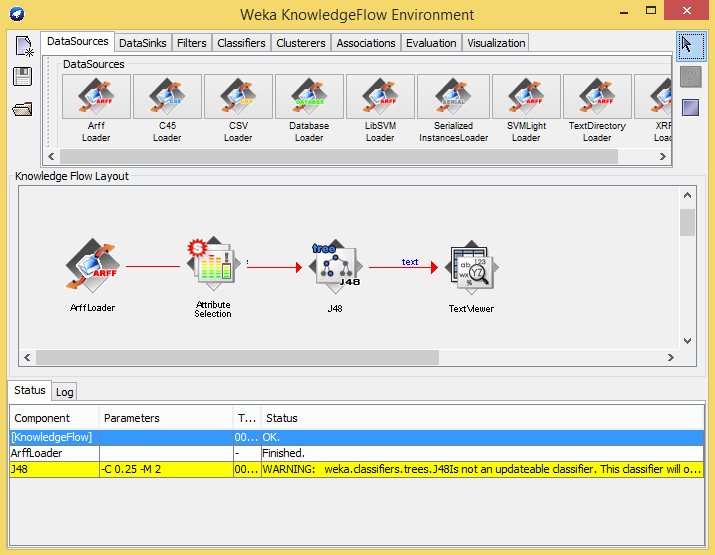
\includegraphics[width=10cm,height=7cm]{images/modo2}}
	\caption {Captura de tela da interface \textit{KnowledgeFlow} do Weka.}
	\label{modo2}
\end{figure}

A opção \textit{Experimenter}, mostrada na Figura \ref{modo3}, tem por objetivo facilitar a identificação de quais métodos e parâmetros nas técnicas de classificação e regressão são mais adequados para determinado problema. A interface foi desenvolvida com o intuito de facilitar ao usuário a comparação de várias técnicas de aprendizagem, tornando mais fácil a execução de classificadores e filtros com diferentes definições de parâmetros sobre um conjunto de dados, a coleta de estatísticas de desempenho e a execução de testes significativos. 

\begin{figure}[!htb]
	\centering
	{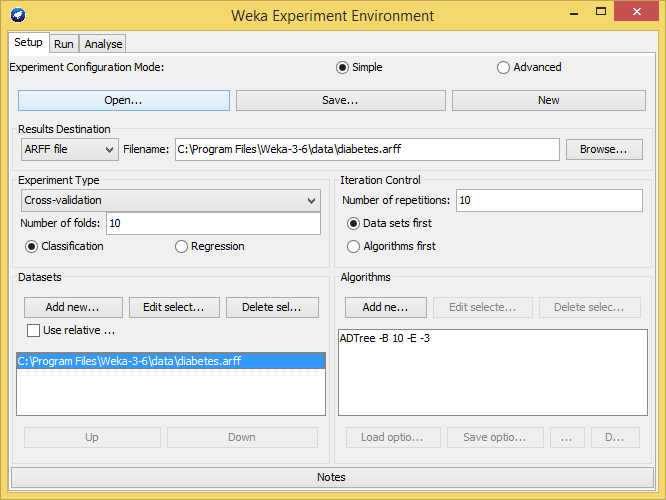
\includegraphics[width=10cm,height=7cm]{images/modo3}}
	\caption {Captura de tela da interface \textit{Experimenter} do Weka.}
	\label{modo3}
\end{figure}
 

Outra possibilidade, além das três interfaces apresentadas anteriormente, é utilizar o Weka pela interface \textit{Simple CLI}, mostrada na Figura \ref{modo4}. A opção \textit{Simple CLI} apresenta dicas de como utilizar o Weka por linha de comando (via \textit{Terminal} no Linux ou \textit{Prompt de Comando} no Windows), e permite ao usuário informar os comandos a serem utilizados na mesma janela.

\begin{figure}[!htb]
	\centering
	{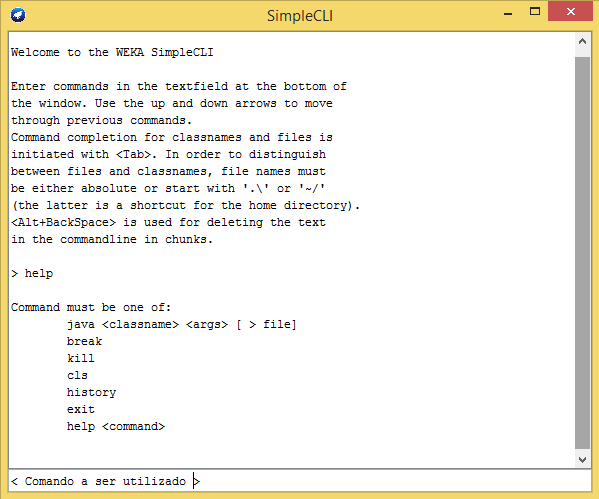
\includegraphics[width=10cm,height=7cm]{images/modo4}}
	\caption {Captura de tela da interface \textit{Simple CLI} do Weka.}
	\label{modo4}
\end{figure}
 
